\documentclass[twocolumn,10pt]{article}
\usepackage[utf8]{inputenc}
\usepackage[T1]{fontenc}
\usepackage{lmodern}
\usepackage[margin=0.85in,top=0.9in,bottom=0.9in]{geometry}
\usepackage{amsmath,amssymb}
\usepackage{graphicx}
\usepackage{booktabs}
\usepackage{url}
\usepackage[hidelinks]{hyperref}
% tikz no longer needed: the overview is figures/overview.png

\usepackage{algorithm}
\usepackage{algpseudocode}
\usepackage{caption}
\usepackage{microtype}
\usepackage{xcolor}
\usepackage{listings}
\captionsetup{font=small,labelfont=bf}
\renewcommand{\topfraction}{0.95}\renewcommand{\bottomfraction}{0.6}\renewcommand{\textfraction}{0.05}\renewcommand{\floatpagefraction}{0.75}\setcounter{topnumber}{3}\setcounter{totalnumber}{5}
\lstset{basicstyle=\ttfamily\fontsize{6}{7.2}\selectfont, breaklines=true, breakatwhitespace=false, columns=fullflexible, keepspaces=true, frame=none, xleftmargin=0pt, aboveskip=2pt, belowskip=2pt}
\newcommand{\nModelName}{CompiledCreditLLM-0.8B-UCI}
\newcommand{\nTrees}{113}
\newcommand{\nLeaves}{1469}
\newcommand{\nSplits}{1356}
\newcommand{\nMaxDepth}{4}
\newcommand{\nTestAUC}{0.778}
\newcommand{\nTestAUCLo}{0.762}
\newcommand{\nTestAUCHi}{0.795}
\newcommand{\nTestKS}{0.437}
\newcommand{\nTestKSLo}{0.408}
\newcommand{\nTestKSHi}{0.469}
\newcommand{\nTestPRAUC}{0.546}
\newcommand{\nTestBrier}{0.136}
\newcommand{\nCalibration}{Platt}
\newcommand{\nXGBVersion}{3.1.2}
\newcommand{\nThresholdChecks}{11,959,257}
\newcommand{\nMarginMaxErr}{2.1e-06}
\newcommand{\nQuantBound}{5.7e-08}
\newcommand{\nSignInversions}{0}
\newcommand{\nRankInversions}{59}
\newcommand{\nOrderedPairsM}{450}
\newcommand{\nRegions}{344,106}
\newcommand{\nShapMaxErr}{8.3e-07}
\newcommand{\nShapMeanErr}{1.2e-08}
\newcommand{\nLocalAccuracyFixed}{0}
\newcommand{\nPolicyTestDecline}{440}
\newcommand{\nPolicyTestReview}{1419}
\newcommand{\nPolicyTestControls}{1011}
\newcommand{\nPolicyTestApprove}{1630}
\newcommand{\nOfficialTensors}{488}
\newcommand{\nCompiledTensors}{3,054}
\newcommand{\nRowsTrain}{1390}
\newcommand{\nRowsValidation}{220}
\newcommand{\nRowsRare}{24}
\newcommand{\nRowsSmoke}{5}
\newcommand{\nTeacher}{Qwen/Qwen3-4B-Instruct-2507}
\newcommand{\nTries}{4}
\newcommand{\nTargetsTrain}{1252}
\newcommand{\nTargetsValidation}{206}
\newcommand{\nTargetsRare}{21}
\newcommand{\nTargetsSmoke}{5}
\newcommand{\nFirstTryYield}{82}
\newcommand{\nRejectRule}{285}
\newcommand{\nRejectNumbers}{641}
\newcommand{\nRejectCausal}{0}
\newcommand{\nRejectSentences}{4}
\newcommand{\nLoraParams}{10.8}
\newcommand{\nLoraModules}{186}
\newcommand{\nLoraSteps}{157}
\newcommand{\nLoraMinutes}{21}
\newcommand{\nLoraRank}{16}
\newcommand{\nEvalLoss}{0.135}
\newcommand{\nTotalTensors}{3,542}
\newcommand{\nLanguageTensors}{473}
\newcommand{\nParityRows}{30,000}
\newcommand{\nRefusalClasses}{7}
\newcommand{\nTamperFloatDiff}{8.9e-16}
\newcommand{\nExplIdenticalCPUGPU}{4}
\newcommand{\nWeightGB}{1.84}
\newcommand{\nAdapterSmokeVerified}{4}
\newcommand{\nAdapterSmokeRows}{5}
\newcommand{\nAdapterSmokeRate}{80.0}
\newcommand{\nAdapterSmokeRefusals}{7}
\newcommand{\nAdapterRareevalVerified}{21}
\newcommand{\nAdapterRareevalRows}{21}
\newcommand{\nAdapterRareevalRate}{100.0}
\newcommand{\nAdapterRareevalRefusals}{7}
\newcommand{\nAdapterValidationVerified}{200}
\newcommand{\nAdapterValidationRows}{206}
\newcommand{\nAdapterValidationRate}{97.1}
\newcommand{\nAdapterValidationRefusals}{7}
\newcommand{\nMergedSmokeVerified}{4}
\newcommand{\nMergedSmokeRows}{5}
\newcommand{\nMergedSmokeRate}{80.0}
\newcommand{\nMergedSmokeRefusals}{7}
\newcommand{\nMergedRareevalVerified}{21}
\newcommand{\nMergedRareevalRows}{21}
\newcommand{\nMergedRareevalRate}{100.0}
\newcommand{\nMergedRareevalRefusals}{7}
\newcommand{\nMergedValidationVerified}{202}
\newcommand{\nMergedValidationRows}{206}
\newcommand{\nMergedValidationRate}{98.1}
\newcommand{\nMergedValidationRefusals}{7}
\newcommand{\nRecourseRows}{232}
\newcommand{\nRecourseReachable}{127}
\newcommand{\nRecourseBlocked}{73}
\newcommand{\nRecourseAlreadyBest}{32}
\newcommand{\nRecourseClose}{110}
\newcommand{\nRecourseModerate}{16}
\newcommand{\nRecourseFar}{1}
\newcommand{\nRecourseDeclineRows}{49}
\newcommand{\nRecourseDeclineReachable}{49}
\newcommand{\nRecourseDeclineOneMove}{47}
\newcommand{\nTimeScorerS}{10}
\newcommand{\nTimeCompileS}{10}
\newcommand{\nTimeBaseS}{6}
\newcommand{\nTimeSampleS}{34}
\newcommand{\nTimeLoraMin}{22}
\newcommand{\nTimeAdapterGatesMin}{18}
\newcommand{\nTimeMergeS}{7}
\newcommand{\nTimeMergedGatesMin}{13}
\newcommand{\nTimeVerifyS}{10}
\newcommand{\nTimeTamperS}{213}
\newcommand{\nTimeNotebookMin}{58}
\newcommand{\nTimeTeacherMin}{115}
\newcommand{\nLoadGPUS}{12.1}
\newcommand{\nScoreGPUMs}{137.5}
\newcommand{\nFullGPUS}{2.78}
\newcommand{\nLoadCPUS}{1.4}
\newcommand{\nScoreCPUMs}{47.6}
\newcommand{\nFullCPUS}{41.62}
\newcommand{\nParagraphWords}{124}

\newcommand{\QW}{Qwenderwriter-0.8B}

\title{\textbf{Qwenderwriter: a complete credit decision system, from scorecard to verified explanation, compiled inside one 0.8B language model}}
\author{\begin{tabular}{c@{\hspace{2.5em}}c}
\textbf{Javier Mancilla}\textsuperscript{*\,\dag} & \textbf{Tom\'as Tagliani}\textsuperscript{*}\\
SquareOne Labs & SquareOne Labs\\
\texttt{javier.m@squareonecap.com} & 
\end{tabular}}
\date{}

\begin{document}
\twocolumn[{
\maketitle
\begin{abstract}
\noindent
We present \QW{}, a single language-model file that performs every step of a credit decision: it validates the
application, scores it with a gradient-boosted scorecard, attributes the score to its drivers with exact Shapley values,
applies a written credit policy, computes the smallest behavioural change that would reach a better outcome, writes a
one-paragraph explanation, and stamps the result with a cryptographic receipt. The scorecard, the attribution tables and
the policy are compiled into exact fixed-point tensors and stored next to the weights of Qwen3.5-0.8B, so one
\texttt{from\_pretrained} call loads the whole system and one SHA-256 digest identifies it. The paragraph is the only free
text in the output, and it is released only after a deterministic verifier finds every number, feature and rule in it
licensed by the evidence, so no hallucinated figure, driver or rule reaches the customer. On the public UCI credit-card benchmark the compiled scorecard reproduces the trained booster on
all 30{,}000 rows with zero sign inversions and the booster's held-out ROC-AUC of \nTestAUC{} and KS of \nTestKS{};
the compiled attribution satisfies local accuracy exactly; the released model writes a verified paragraph for
\nMergedValidationRate\% of held-back applications and \nMergedRareevalRate\% of rare-rule applications; it refuses all
seven malformed request classes before the language model is invoked; and it returns byte-identical assessments across
repeats, batch sizes and devices, while a single flipped bit in the compiled region makes it refuse to score. A full
assessment without the paragraph takes \nScoreCPUMs{}~ms on a CPU, the paragraph adds \nFullGPUS{}~s on a desktop GPU, and
the complete build, from raw data to the tested model, runs in under an hour on one workstation. Code, data preparation,
tests and the model are released for non-commercial use.
\end{abstract}
\vspace{1.2em}
}]
\renewcommand{\thefootnote}{\fnsymbol{footnote}}
\footnotetext[1]{SquareOne Labs is a frontier technology lab that applies generative AI, quantum computing, and neuromorphic/thermodynamic computing to real-world problems across industries, with a strong focus on financial services. Its work spans three major areas: credit risk and portfolio intelligence, proprietary domain-specific AI models, and responsible AI governance. These rest on a base of in-house IP and a team that takes solutions from research to production.}
\footnotetext[2]{Corresponding author. Javier Mancilla conceived and built \QW{} and owns the code and the released model, which are published from the author's personal GitHub account; Tom\'as Tagliani acted as pair reviewer of the design, the code and the manuscript. Both authors are affiliated with SquareOne Labs.}
\renewcommand{\thefootnote}{\arabic{footnote}}\setcounter{footnote}{0}

\begin{figure*}[!t]
\centering
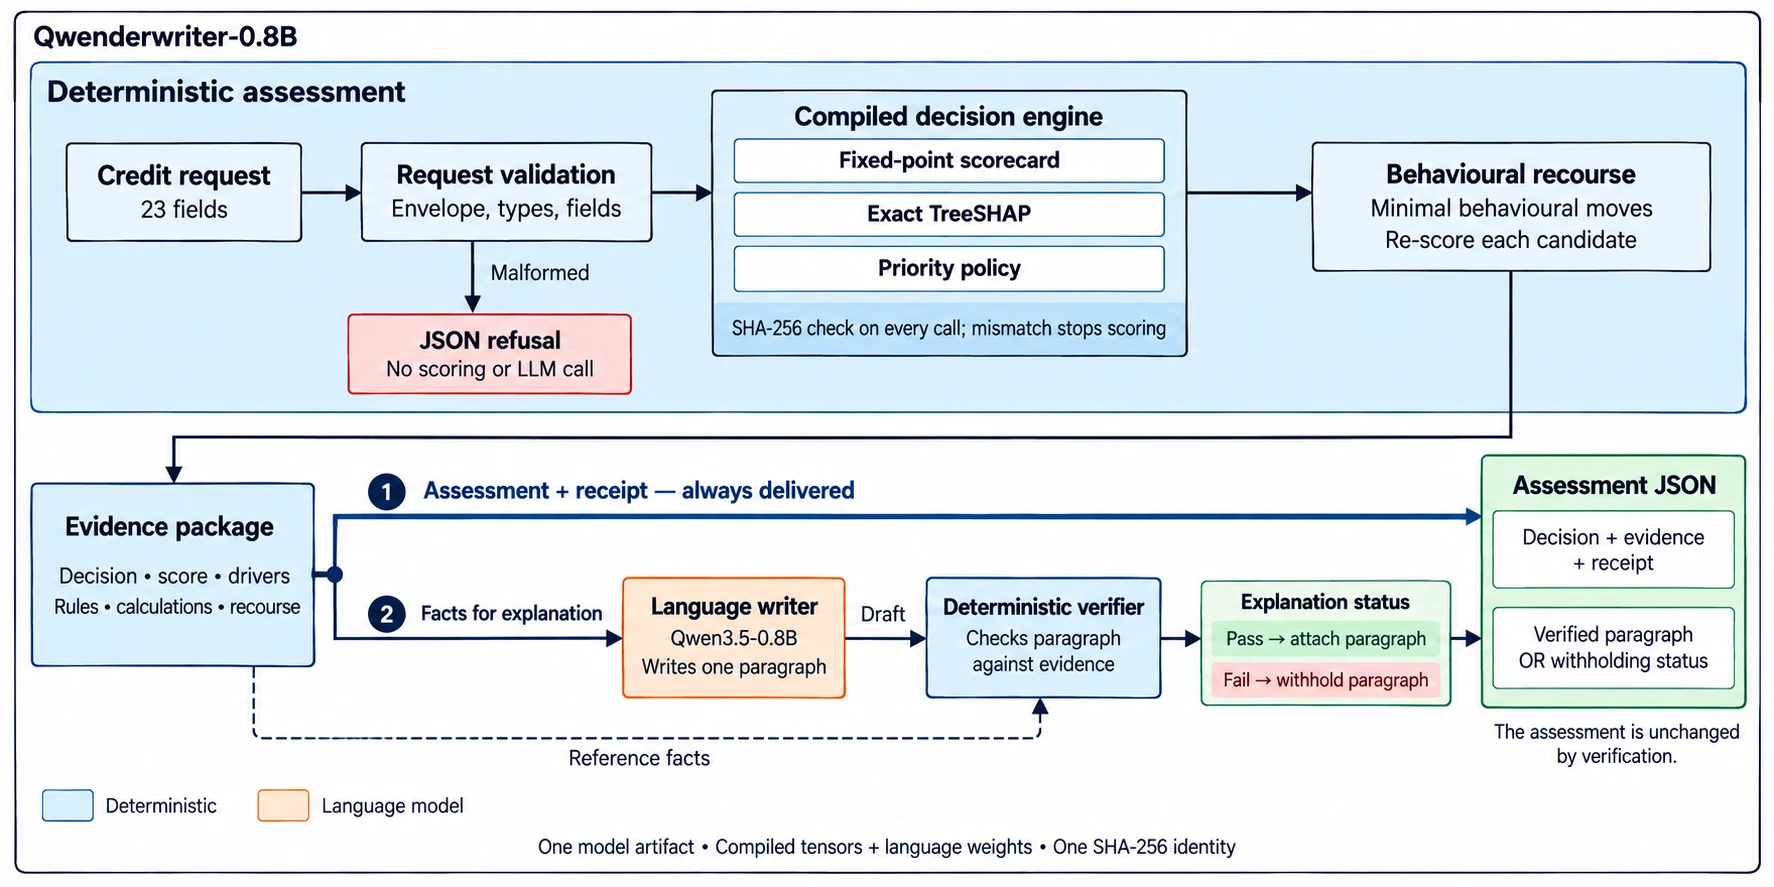
\includegraphics[width=\textwidth]{figures/overview.png}
\caption{Overview of \QW{}. The upper band is the deterministic assessment: the request is validated (a malformed request receives an exact JSON refusal and nothing else runs), scored by the compiled decision engine (fixed-point scorecard, exact TreeSHAP, priority policy, with a SHA-256 check of the compiled buffers on every call) and completed with behavioural recourse. The evidence package feeds two outputs: the assessment with its receipt, which is always delivered, and the facts from which the language writer drafts one paragraph that a deterministic verifier checks against the same evidence before it is attached or withheld. One model artefact holds the compiled tensors and the language weights under one identity.}
\label{fig:overview}
\end{figure*}

\section{Introduction}

A credit decision has two audiences. The borrower and the analyst want a readable account of what was decided, why, and
what would change it. The risk function and the auditor want the number, the rule that fired, and proof that nothing
between the model and the decision letter altered either. Large language models serve the first audience well and the second
poorly: they write fluent paragraphs, but generated text is known to depart from its source, a failure documented as
hallucination~\cite{maynez2020faithfulness,ji2023hallucination}; in a decision letter that departure takes the form of invented
percentages, rounded numbers that must not be rounded, and associations described as causes. The usual remedy is a pipeline: a
scoring service, an explanation library, a policy engine, a prompt that pastes their outputs into a language model, and
a filter on the way out. Each component is reasonable. The difficulty lies in the composition: the components drift apart, the
prompt becomes the de facto specification, and the paragraph that reaches the customer is the one artefact that cannot
be traced to a specific model version. A language model asked to explain a decision that was already made adds a failure
mode of its own: it rationalises the outcome it is handed, selects or invents evidence that supports it, offers no
guarantee that the facts it cites are the ones that decided the case, and leaves out the pipeline logic and the policy rules
that actually produced the decision.

\QW{} collapses that pipeline into one file (Figure~\ref{fig:overview}). The scorecard, its attribution and the policy are compiled into tensor
buffers and stored in the same safetensors file as a small language model. The model class that loads the file runs the
scorecard as tensor arithmetic, re-checks a cryptographic receipt of the compiled buffers on every call, derives the
policy outcome and the recourse options, and then asks the language layers to write one paragraph from a fixed fact
sheet. The paragraph is released only if a verifier finds every number, feature name and rule phrase in it licensed by the
evidence. The result is one artefact with one identity: whatever version of the file produced a decision letter also produced the
score, the attribution, the policy outcome and the receipt in that letter.

Three design choices carry the weight.

\noindent (i) \emph{Exactness}: trees are evaluated on an integer lattice where the branch
predicate is an identity, not a float comparison, so the compiled score is the trained booster's score, not an
approximation of it (Section~\ref{sec:compile}).

\noindent (ii) \emph{Separation of arithmetic and prose}: the score, the drivers, the
policy and the recourse come from the compiled buffers; the transformer only writes, and the tamper tests make the
separation measurable (Section~\ref{sec:tamper}).

\noindent (iii) \emph{Verification before release}: the paragraph is checked against the
numbers that produced it, and when it fails the decision is delivered without it (Section~\ref{sec:writer}).

Section~\ref{sec:output} shows the raw output of the model on one application. Section~\ref{sec:method} describes how
each block is built. Section~\ref{sec:experiments} reports the evidence on the benchmark, including the machine and the
time each stage took. Section~\ref{sec:discussion} explores what the package has to offer a lender, how several scorecards can
share one file, and what remains to be done before any of this reaches a real book. Caveats are collected in
Section~\ref{sec:limits}.

\section{Output of the model}
\label{sec:output}

Figure~\ref{fig:raw} shows one application from the benchmark and the complete answer, exactly as the model returns it.
The input is the applicant's 23 fields: credit limit, four demographic fields, six monthly repayment statuses, six
statement balances and six payment amounts. The output is one JSON document with nine blocks.

\begin{itemize}\setlength\itemsep{1pt}
\item \textbf{decision}: the outcome, the level that decided it and the rule that controlled it. In this example a policy rule,
  severe delinquency, is triggered at the highest priority level and the application is declined.
\item \textbf{model}: the probability of default from the compiled scorecard, its risk band and the raw margin. The
  probability is printed to twelve digits because the receipt below quotes it.
\item \textbf{policy}: every rule that was active at every level, not only the one that won, so a reviewer sees that
  three soft controls and a review trigger were also live.
\item \textbf{drivers}: the two strongest risk-increasing and risk-decreasing features with their exact Shapley
  contributions to the margin. They come from the same compiled model as the score, so a driver can never contradict it.
\item \textbf{calculations}: the thirteen figures the policy rules evaluate, in the units those rules use.
\item \textbf{data\_quality}: input conditions the policy rules flagged, phrased for a human.
\item \textbf{recourse}: the most useful block for the applicant. In this example the applicant is one step away from approval with controls
  (bring the six repayment statuses current; the probability would fall from 69.9\% to 11.7\%) and two steps away from a
  standard approval. Only behavioural fields may change; demographic fields never do.
\item \textbf{explanation}: the one paragraph the language layers wrote, and its verification status. Every number and
  name in it was checked against the blocks above before it was released.
\item \textbf{receipt}: a byte-exact line with the fixed-point margin, the probability, the outcome, band, flags,
  triggers, calculations and drivers, plus the policy identifier. An auditor can reproduce the whole decision from this
  line and the model file, without running the language layers.
\end{itemize}

A malformed request never reaches any of this. The lower-left panel of Figure~\ref{fig:raw} shows the answer to a request
that tries to override the outcome: an exact JSON refusal, with the language model not invoked. Six other classes
(unsupported action, missing field, non-integer value, duplicate field, value outside 64 bits, evidence line that does
not match) receive the same treatment.

\begin{figure*}[!tp]
\begin{minipage}[t]{0.40\textwidth}
\textbf{Request} (one of the released examples)
\begin{lstlisting}
{"action": "ASSESS",
 "credit": {"LIMIT_BAL": 200000, "SEX": 2, "EDUCATION": 2,
   "MARRIAGE": 1, "AGE": 39,
   "PAY_0": 3, "PAY_2": 2, "PAY_3": 2, "PAY_4": 2, "PAY_5": 2,
   "PAY_6": 0,
   "BILL_AMT1": 117868, "BILL_AMT2": 114483, "BILL_AMT3": 118855,
   "BILL_AMT4": 125357, "BILL_AMT5": 121853, "BILL_AMT6": 124731,
   "PAY_AMT1": 0, "PAY_AMT2": 6216, "PAY_AMT3": 10000,
   "PAY_AMT4": 0, "PAY_AMT5": 5000, "PAY_AMT6": 4552}}
\end{lstlisting}
\vspace{4pt}
\textbf{Answer to the same request with an added \texttt{"override"} key}
\begin{lstlisting}
{"protocol": "compiled-credit-llm/assessment-v1",
 "status": "REFUSE",
 "refusal_class": "OVERRIDE_ATTEMPT",
 "reason": "Checkpoint evidence and policy outcomes cannot be overridden.",
 "language_model_invoked": false,
 "receipt": "RECEIPT1|status=REFUSE|e=OVERRIDE_ATTEMPT|n=Checkpoint evidence and policy outcomes cannot be overridden.|d=SYNTHETIC_NONREGULATORY_ASSOCIATIVE_NOT_CAUSAL"}
\end{lstlisting}
\vspace{4pt}
\small The answer on the right is the file's complete output for the request above, produced by one call,
\texttt{model.assess\_credit(request, tokenizer)}. Values are those of the released model; the paragraph is the language
layers' own text after verification. The long \texttt{boundary} string is abridged here; nothing else is.
\end{minipage}\hfill
\begin{minipage}[t]{0.57\textwidth}
\textbf{Assessment}
\begin{lstlisting}
{"protocol": "compiled-credit-llm/assessment-v1", "status": "OK",
 "decision": {"outcome_code": "DD", "outcome": "demonstration decline", "level": "hard",
   "controlling_rules": ["severe delinquency"],
   "note": "first active level in priority order hard > review > soft > approve"},
 "model": {"probability": "0.698978159399", "probability_pct": "69.9%",
   "risk_band": "elevated", "raw_margin": 0.842437},
 "policy": {"id": "UCI_DEMO_POLICY_v1", "priority": ["hard", "review", "soft", "approve"],
   "active": {"hard": ["severe delinquency"],
     "review": ["multiple soft controls require review"],
     "soft": ["repeated delinquency", "low payment coverage", "elevated model risk"]}},
 "drivers": {
   "increasing_risk": [
     {"feature": "Most recent repayment status", "code": "PAY_0", "contribution": 1.566583},
     {"feature": "Repayment status three months ago", "code": "PAY_3", "contribution": 0.236006}],
   "decreasing_risk": [
     {"feature": "Payment amount three months ago", "code": "PAY_AMT3", "contribution": -0.111109},
     {"feature": "Credit limit amount", "code": "LIMIT_BAL", "contribution": -0.108503}]},
 "calculations": {"current_utilization_pct": 58.93, "max_utilization_pct": 62.67,
   "avg_utilization_pct": 60.26, "delinquent_statuses": 5, "repeated_delinquency": true,
   "max_severity": 3, "payment_coverage_pct": 3.56, "balance_trend_pct": -3.44,
   "bill_dispersion": 3455, "payment_dispersion": 2863, "zero_payment_stress": false,
   "positive_bill_total": 723147, "payment_total": 25768},
 "data_quality": ["a repayment code is undocumented in the UCI source"],
 "recourse": {"current_outcome": "demonstration decline", "current_outcome_code": "DD",
   "scope": "behavioural fields only: repayment statuses, statement balances, payments",
   "non_behavioural_blockers": [], "status": "REACHABLE",
   "next_better": {"outcome": "approval with controls", "outcome_code": "AC", "moves_needed": 1,
     "moves": ["all six repayment statuses paid on time (no month in delay)"],
     "fields_changed": 5, "model_after": {"risk_band": "low", "probability_pct": "11.7%"}},
   "best_reachable": {"outcome": "standard demonstration approval", "outcome_code": "AS",
     "moves_needed": 2,
     "moves": ["all six repayment statuses paid on time (no month in delay)",
       "total payments over the six months of at least 72,315 instead of 25,768 (payment coverage 10.00% of positive bills)"],
     "fields_changed": 6, "model_after": {"risk_band": "low", "probability_pct": "9.8%"}},
   "proximity": "close"},
 "explanation": "The decision is demonstration decline controlled by severe delinquency. The model assigns a 69.9% probability of DEFAULT, placing the risk_band in elevated. Key risk-increasing drivers include most recent repayment status and repayment status three months ago, while risk-decreasing factors are payment amount three months ago and credit limit amount. Calculations show current utilization at 58.93%, max at 62.67%, five delinquent statuses, payment coverage at 3.56%, and a balance trend of -3.44%. A data-quality flag notes a repayment code is undocumented in the UCI source. The case is close to approval with controls, requiring all six repayment statuses to be paid on time with no month in delay. The probability is an association from a benchmark model, not a cause and not a guarantee.",
 "explanation_status": "VERIFIED",
 "boundary": "Synthetic demonstration policy UCI_DEMO_POLICY_v1 on the historical 2005 UCI benchmark; [...] not a lending, regulatory or adverse-action decision.",
 "receipt": "RECEIPT1|p=UDP1|s=842436674|q=0.698978159399|o=DD|b=E|f=UR|t=DS,RM,CD,CP,CE|c=cu:5893,mu:6267,au:6026,dc:5,rd:1,ms:3,pc:356,bt:-344,bd:3455,pd:2863,zs:0,pb:723147,pt:25768|xp=PAY_0:1566582684,PAY_3:236005770|xn=PAY_AMT3:-111109176,LIMIT_BAL:-108502860|r=DS|d=SYNTHETIC_NONREGULATORY_ASSOCIATIVE_NOT_CAUSAL"}
\end{lstlisting}
\end{minipage}
\caption{A raw request and the raw answer of \QW{}. One applicant from the UCI benchmark is declined by a policy rule, is shown to be one behavioural step away from approval with controls, and receives a verified paragraph and a receipt that reproduces the decision. A request that tries to override the outcome is refused before any model code runs.}
\label{fig:raw}
\end{figure*}

\section{Related work}

Compiling tree ensembles to tensor programs for serving is established; Hummingbird~\cite{nakandala2020hummingbird}
translates trees into GEMM and gather operations for GPUs. Our compilation differs in purpose: we trade speed for
exactness and auditability, with integer-lattice predicates, fixed-point accumulation at a declared scale, a proof of
threshold equivalence over every observed value, and a receipt over the compiled state.

TreeSHAP~\cite{lundberg2020treeshap} gives exact Shapley attributions for tree ensembles in polynomial time. We do not
re-implement the algorithm; we compile its output. The observation that attribution is constant on every cell of the
product of a tree's split thresholds lets us tabulate it per tree at compile time and reduce inference to a table lookup (a tensor gather: the row of a precomputed
table is read by index instead of being computed), with an integer correction that makes local accuracy exact.

Counterfactual explanations~\cite{wachter2018counterfactual} and actionable recourse~\cite{ustun2019recourse,karimi2022survey}
consider what change would flip a decision. Our recourse engine is deliberately narrow: a small set of policy-derived moves
over behavioural fields, exhaustively re-scored, with immutable and protected fields excluded. The hidden assumptions
catalogued by Barocas et al.~\cite{barocas2020hidden} apply and are stated in the output itself.

Rudin's case for interpretable models in high-stakes decisions~\cite{rudin2019stop} motivates keeping the decision in an
auditable deterministic scorecard. Our design keeps the decision in a tree ensemble and a rule table and restricts the opaque component
to prose about them. Faithfulness of generated text to its source~\cite{maynez2020faithfulness} is enforced here by a
verifier with a licensed vocabulary of numbers and names, rather than measured after the fact.

\section{Method}
\label{sec:method}

\subsection{Data}

The UCI ``default of credit card clients'' dataset (UCI repository id 350)~\cite{uci350,yeh2009comparisons} was collected
by a Taiwanese card issuer in 2005 and released by I-Cheng Yeh. It has 30{,}000 clients and 23 attributes: the credit
limit, four demographic fields (sex, education, marital status, age), six monthly repayment statuses from April to
September 2005 (coded from paid duly to nine months of delay), six monthly statement balances and six monthly payment
amounts in New Taiwan dollars. The label is whether the client defaulted on the next month's payment; 22.1\% did. It is
the most widely used public credit benchmark, it has no application ordering or timestamps beyond the six months, and its
repayment codes contain undocumented values (such as $-2$ and $0$) that a careful policy must flag rather than silently
interpret.

We use a client-level stratified split: train 18{,}000, validation 4{,}500, calibration 3{,}000, test 4{,}500. The test
split is read once, by the scorecard's locked evaluation; no explanation-side step reads it.

\subsection{Request path}

A request is a mapping from the 23 attribute names to integers or explicit nulls. Figure~\ref{fig:overview} shows the path
from request to answer. Everything but the language writer is deterministic tensor or rule code shipped with the model class.

\subsection{Compiling the scorecard to exact tensors}
\label{sec:compile}

Let $x \in \mathbb{Z}^{d}$ be a feature vector on an integer lattice with declared per-feature scales (scale 1 for the UCI
fields) and let $m \in \{0,1\}^{d}$ be its missing mask. For an integer threshold $t$ and a feature value $x_j$,
\begin{equation}
\min\!\big(\mathrm{relu}(t - x_j),\, 1\big) \;=\; [\,x_j < t\,],
\label{eq:pred}
\end{equation}
exactly, including equality going right as in the XGBoost implementation~\cite{chen2016xgboost,xgboostcode}. A native floating threshold $\tau$ on a
feature with scale $s$ is normalised to $t = \lceil \tau s \rceil$, which preserves~\eqref{eq:pred} for every lattice
value; the compiler proves this over every observed value and five integers around every boundary
(\nThresholdChecks{} comparisons on the UCI model, zero mismatches). Missing values follow the tree's default direction:
with $\ell = 1$ for default-left, the left gate is $\min(\ell(p + m_j), 1) + (1-\ell)\,\mathrm{relu}(p - m_j)$ with $p$
the predicate of~\eqref{eq:pred}.

Each leaf stores its root-to-leaf path as a row of up to $D$ gates (feature index, threshold, default direction, edge
side). A leaf is active when all its gates are active,
\begin{equation}
a_\ell = \min\!\Big(\mathrm{relu}\Big(\sum_{k=1}^{D} g_{\ell k} - |\pi_\ell| + 1\Big),\, 1\Big),
\end{equation}
and exactly one leaf per tree is active. Leaf values are quantised at scale $10^{9}$, so the margin is an integer
accumulated by a matrix product in float64, which carries integers below $2^{53}$ exactly. The per-leaf quantisation error
is at most $0.5\times10^{-9}$ and the margin error is bounded by $(T+1)\times 0.5\times10^{-9}$ with $T$ trees
(\nQuantBound{} for the UCI model).

\subsection{Exact TreeSHAP as a lookup}

TreeSHAP attribution is not constant across the rows that reach one leaf, because the cold subtrees of the path matter.
It is constant across every cell of the product of a tree's split thresholds, because such a cell fixes every branch
decision in the tree. For each tree the compiler enumerates these cells (\nRegions{} in total for the UCI model),
queries the native booster once per cell with a representative row, quantises the $d$ contributions at $10^{9}$, and adds
the sub-unit rounding residual to the largest-magnitude component so that
\begin{equation}
\sum_{j=1}^{d} \phi_{j}(x) + \phi_0 = \text{margin}(x)
\end{equation}
holds exactly in integer units for every cell, hence for every input. At inference each tree computes a mixed-radix cell
index with $d'$ threshold comparisons ($d'$ the features the tree uses) and gathers its contribution vector; the sum over
trees is the attribution.

\subsection{Policy in integer arithmetic}

The demonstration policy computes thirteen quantities with floor division in basis points (current, maximum and average
utilization, delinquency count and maximum severity, payment coverage, bill trend, two dispersions, zero-payment stress,
positive bill total, payment total), six flags (missing input, contract violation, out of development range, unknown
demographic category, undocumented repayment code, type invalid), four risk bands on the raw margin, and fifteen
triggers, and resolves them by first match: invalid input, decline, manual review, approval with controls, standard
approval. Both the trigger vector and the final-reason vector are returned, so the priority never hides which conditions
were active. Thresholds are declared assumptions, development bounds come from non-test rows, and no threshold was fitted
to labels. All of it is \texttt{int64} tensor code on buffers the verifier hashes; an independent NumPy oracle reproduces
it on all 30{,}000 rows in the compile audit and again in the verification report.

\subsection{Receipt, self-checks and refusals}

The config of the file carries a SHA-256 digest of the compiled state: every buffer's name, dtype, shape and raw bytes in
sorted order. Each scoring call recomputes the digest (cached by tensor version, so an in-place change invalidates the
cache) and raises if it differs. The call also recomputes grade and decision from the margin, checks the local-accuracy
identity, exactly one risk band and exactly one outcome, and probability bounds. The evidence line that feeds every later
stage is serialised only from a result that passed these checks, and the receipt in the output is a byte-exact rewrite of
that line.

Before any of this, the request envelope is validated with a fixed precedence: an override key, an unsupported action or
key, a missing field set, a non-integer or Boolean value, a duplicate field, a value outside signed 64 bits, and a supplied
evidence line that does not match the recomputed one. Each class returns an exact JSON refusal; none reaches the scorecard
or the language layers. An explicit null is not a malformed request: it is a policy input that yields the invalid-input
outcome with the missing field named.

\subsection{Recourse}

Candidate single moves are derived from the policy rules' thresholds: all six statuses on time; no status later than one month;
one delayed month only; total payments raised to the coverage threshold; every balance held under the high or extreme
utilization cap; the most recent balance held under the rising-trend cap. Combinations of up to three moves are re-derived
on the progressively modified vector so they compose exactly, and every candidate is re-scored by the compiled scorecard.
The engine reports the smallest improvement with the fewest moves, the best reachable outcome with the fewest moves, the
number of fields changed, and the band and probability after the change, with a proximity label of close, moderate or far.
Only repayment statuses, balances and payments move; a missing field, a contract violation, an unknown category or an
out-of-range value is reported as a non-behavioural blocker instead of a move.

\subsection{The explanation writer}
\label{sec:writer}

The language layers receive a compact JSON of facts (decision and controlling rules, probability and band, active rules
per level, driver labels without codes or contributions, the thirteen calculations, data-quality phrases, and the
proximity block of the recourse result) and a writing brief, and return one paragraph. The verifier then requires the
exact outcome phrase of the policy (for example ``declined''), every controlling-rule phrase verbatim, the probability and the band, the association caveat and the
recourse statement; it forbids any number not in the licensed set (the probability in its allowed forms, the calculations
in theirs, small ordinals, and the exact numbers of the recourse moves), any feature label not among the drivers or the
recourse text, raw feature codes, quotation marks, brackets and currency signs, and a list of causal, legal and guarantee
phrasings, including inverted readings of the probability. A paragraph that fails is withheld and the violations are
listed; the decision is delivered regardless.

Training targets were written by a teacher model from exactly the facts JSON and brief the file sends at serving time,
sampled up to \nTries{} times per row and kept only if the verifier accepted them (Algorithm~\ref{alg:teach}). The 0.8B
backbone was then adapted with LoRA~\cite{hu2022lora} on the language layers only; the compiled buffers were hashed before
and after. Teacher-forced loss was recorded and never used for selection: the adapter and the merged file were judged by
free generation on the real request path, including the seven refusals with the language layers forbidden.

\begin{algorithm}[t]
\caption{Verifier-filtered targets and gated adaptation}
\label{alg:teach}
\begin{algorithmic}[1]
\Require development rows $R$, compiled file $C$, teacher $T$, verifier $V$, tries $k$
\For{each row $r \in R$}
  \State $e \gets C.\mathrm{evidence}(r)$;\quad $\rho \gets C.\mathrm{recourse}(r)$
  \State $f \gets \mathrm{facts}(e, \rho)$ \Comment{labels only; no codes, no raw contributions}
  \For{$i = 1 \ldots k$}
    \State $p \gets T(f)$
    \If{$V(p, e, \rho) = \emptyset$} keep $(f, p)$; \textbf{break} \EndIf
  \EndFor
\EndFor
\State adapt the language layers of $C$ on the kept pairs with LoRA; assert $\mathrm{hash}(C.\mathrm{compiled}) $ unchanged
\State gate by free generation on the real path: verified rate on held-back rows, refusals $= 7/7$ with no model call
\State merge the adapter; re-run the gate, verification, tamper and determinism tests on the merged file
\end{algorithmic}
\end{algorithm}

\section{Experiments}
\label{sec:experiments}

\subsection{Scorecard}

A bounded search of twelve XGBoost configurations (version \nXGBVersion{}) on the validation split selects depth
\nMaxDepth{} with \nTrees{} trees (\nLeaves{} leaves, \nSplits{} splits); a frozen rule keeps \nCalibration{}
calibration. Held-out ROC-AUC is \nTestAUC{} (95\% bootstrap interval \nTestAUCLo{} to \nTestAUCHi{}), KS \nTestKS{}
(\nTestKSLo{} to \nTestKSHi{}), PR-AUC \nTestPRAUC{}, Brier \nTestBrier{} (Figure~\ref{fig:scorer}a). These are
standard numbers for this benchmark; the scorecard is not the contribution, the packaging around it is.

Under the demonstration policy the 4{,}500 test rows resolve to \nPolicyTestDecline{} declines, \nPolicyTestReview{}
manual reviews, \nPolicyTestControls{} approvals with controls and \nPolicyTestApprove{} standard approvals, a
distribution that matches the training split closely (Figure~\ref{fig:scorer}b).

\begin{figure}[t]
\centering
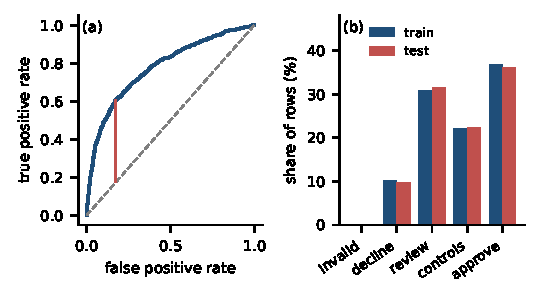
\includegraphics[width=\columnwidth]{figures/scorer_policy.pdf}
\caption{(a) Held-out ROC curve of the booster; the vertical segment marks the KS point. (b) Share of rows per policy outcome on the training and test splits; the policy behaves the same on data it has not seen.}
\label{fig:scorer}
\end{figure}

\subsection{Is the compiled scorecard the trained model?}

Figure~\ref{fig:parity} addresses this question, and it matters because every later guarantee depends on it: if the
tensors inside the file computed something slightly different from the validated booster, the receipt would certify the
wrong model. Panel (a) plots the margin produced by the compiled tensors against the margin produced by XGBoost itself, for
the held-out rows; every point lies on the diagonal. Panel (b) is the histogram of the absolute difference over all 30{,}000
rows: the largest is \nMarginMaxErr{}, about two millionths of a logit. The compilation's own rounding bound is
\nQuantBound{}, forty times smaller, so the visible difference is the booster's float32 accumulation order, not the
compilation. The consequence is exact in the quantities a lender cares about: \nSignInversions{} rows change the sign of
the margin, the 30{,}000 rows keep their order except for \nRankInversions{} pairs out of \nOrderedPairsM{} million
whose margins differ by less than the float32 noise, and ROC-AUC and KS on the test split are identical to the printed
precision. Attribution behaves the same way: local accuracy holds with \nLocalAccuracyFixed{} residual units on every row,
and the largest difference from native float32 TreeSHAP is \nShapMaxErr{} (mean \nShapMeanErr{}).

\begin{figure}[t]
\centering
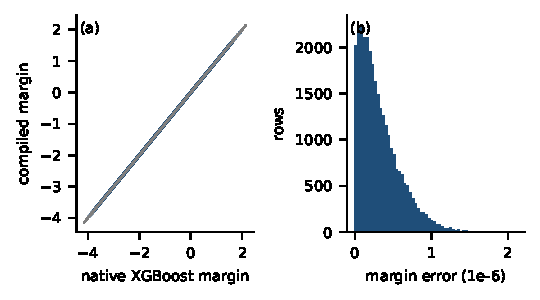
\includegraphics[width=\columnwidth]{figures/parity.pdf}
\caption{The compiled scorecard against the native booster. (a) Margin from the tensors inside the file versus the margin from XGBoost, held-out rows: every point is on the diagonal. (b) Absolute difference on all 30{,}000 rows, in millionths of a logit; the spread is the booster's own float32 accumulation, forty times larger than the compilation's rounding bound. Zero sign inversions, identical ROC-AUC and KS.}
\label{fig:parity}
\end{figure}

\subsection{The file}

The base file holds the \nOfficialTensors{} official backbone tensors unchanged (each hashed before and after packaging)
and \nCompiledTensors{} compiled buffers in one safetensors file of \nWeightGB{}~GB; the released file differs only in the
adapted language tensors. Verification reloads it strictly, checks the compiled digest, scores all \nParityRows{} rows
against the base file (every tensor and label field exact), checks the policy against the oracle on every row, and runs
the seven refusal classes with generation forbidden (\nRefusalClasses{}/7, zero calls).

\subsection{Explanation writer}

Development rows were sampled from the train split (\nRowsTrain{} rows) and the validation split (\nRowsValidation{}
validation rows, \nRowsRare{} rare-rule rows carrying unknown-category, zero-payment and extreme-utilization triggers,
and a smoke set of \nRowsSmoke{} rows with one row per outcome), with variants that create cases a natural row cannot:
explicit nulls and contract violations for invalid input, out-of-range ages for manual review. The teacher
(\nTeacher{}) produced a verified paragraph on the first try for \nFirstTryYield\% of rows; after \nTries{} tries
\nTargetsTrain{} training targets, \nTargetsValidation{} validation targets, \nTargetsRare{} rare-rule targets and
\nTargetsSmoke{} smoke targets remained. The verifier's most frequent objections were an unlicensed number
(\nRejectNumbers{} drafts) and a controlling rule not quoted verbatim (\nRejectRule{}); a wrong sentence count
(\nRejectSentences{}) and length (1) were rare (Figure~\ref{fig:gates}b). A 4B instruction model therefore invents
or rounds a number in roughly one draft out of six even when every licensed number is provided to it, which is the
behaviour the verifier is designed to detect.

LoRA rank \nLoraRank{} on \nLoraModules{} linear modules (\nLoraParams{}M parameters), one pass of \nLoraSteps{}
steps in \nLoraMinutes{} minutes, final held-back loss \nEvalLoss{}.

\paragraph{Evaluation of the writer.} Loss on teacher text sheds very little light on what a model writes when it is free to
do so, so the writer is judged only by free generation on the real request path (Table~\ref{tab:gates},
Figure~\ref{fig:gates}a). Each held-back application is sent through the released code exactly as a user would send it;
the model writes its paragraph; the verifier decides. ``Verified'' means the paragraph quoted the outcome, the controlling
rule, the probability and the band, used no number and no feature name outside the licensed set, and made no causal or
guarantee claim. On \nMergedValidationRows{} held-back applications the released file writes a verified paragraph
\nMergedValidationRate\% of the time, and on the \nMergedRareevalRows{} applications that trigger rare rules (unknown
category, zero payments, extreme utilization) it does so every time. The table also reports the seven malformed request
classes: all seven were refused with the exact expected JSON and the language layers were never called. The small smoke
set serves to detect regressions rather than to measure performance; one of its five rows is a paragraph the verifier withheld, which
is the designed behaviour, not an error. In every withheld case the decision, the numbers and the receipt were delivered
unchanged, because none of them come from the language layers.

\begin{table}[t]
\centering\footnotesize\setlength{\tabcolsep}{4pt}
\caption{Free generation on the real request path, before and after merging the adapter into the file. Verified: the paragraph passed every verifier rule. Refusals: the seven malformed request classes, all refused with the exact JSON and zero language-model calls.}
\label{tab:gates}
\begin{tabular}{llrrr}
\toprule
weights & held-back rows & verified & rate (\%) & refusals \\
\midrule
adapter & smoke (\nAdapterSmokeRows) & \nAdapterSmokeVerified & \nAdapterSmokeRate & \nAdapterSmokeRefusals/7 \\
adapter & rare rules (\nAdapterRareevalRows) & \nAdapterRareevalVerified & \nAdapterRareevalRate & \nAdapterRareevalRefusals/7 \\
adapter & validation (\nAdapterValidationRows) & \nAdapterValidationVerified & \nAdapterValidationRate & \nAdapterValidationRefusals/7 \\
merged & smoke (\nMergedSmokeRows) & \nMergedSmokeVerified & \nMergedSmokeRate & \nMergedSmokeRefusals/7 \\
merged & rare rules (\nMergedRareevalRows) & \nMergedRareevalVerified & \nMergedRareevalRate & \nMergedRareevalRefusals/7 \\
merged & validation (\nMergedValidationRows) & \nMergedValidationVerified & \nMergedValidationRate & \nMergedValidationRefusals/7 \\
\bottomrule
\end{tabular}
\end{table}

\begin{figure}[t]
\centering
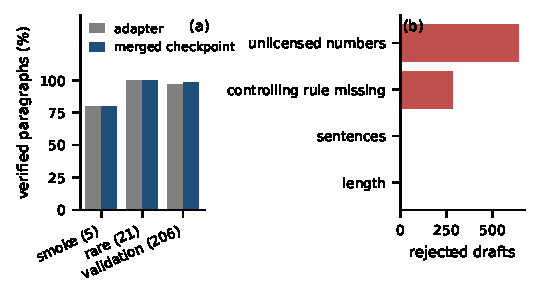
\includegraphics[width=\columnwidth]{figures/gates.pdf}
\caption{(a) Share of held-back applications for which the writer produced a paragraph that passed the verifier, before (adapter) and after (merged) folding the adapter into the file; merging loses nothing. (b) Why the verifier rejected teacher drafts while the training targets were written: numbers the teacher was not licensed to use dominate.}
\label{fig:gates}
\end{figure}

\subsection{Recourse}

Figure~\ref{fig:recourse} summarises the recourse block over the \nRecourseRows{} gated development rows. For
\nRecourseAlreadyBest{} the current outcome is already the best the policy rules offer. For \nRecourseBlocked{} a better
outcome is not reachable by behaviour: a missing field, an unknown demographic category or a value outside the development
range routes the case to human review whatever the applicant does, and the engine says so instead of inventing a move.
For \nRecourseReachable{} a better outcome is reachable, and for \nRecourseClose{} of those a single move suffices. All
\nRecourseDeclineRows{} declined applicants in the set are reachable, \nRecourseDeclineOneMove{} of them with one step,
most often bringing the repayment statuses current. These are exact statements about the compiled scorecard and the
policy, re-scored by the same buffers that produced the decision, and they are what makes a decline letter
actionable.

\begin{figure}[t]
\centering
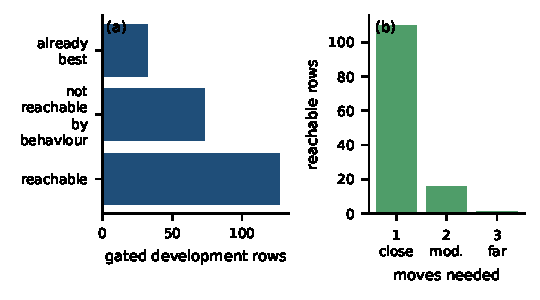
\includegraphics[width=\columnwidth]{figures/recourse.pdf}
\caption{Recourse over the gated development rows. (a) How many applicants are already at the best outcome, are blocked by a non-behavioural condition, or can reach a better outcome by changing repayment behaviour. (b) Among the reachable ones, how many moves the next better outcome needs; most need one.}
\label{fig:recourse}
\end{figure}

\subsection{Tamper and determinism}
\label{sec:tamper}

Table~\ref{tab:tamper} lists nine tests on the released file. The first five check whether the file notices when its
compiled region is altered. Changing one tree leaf, one policy bound or the expected digest in memory, or flipping one bit
inside the compiled region of the file on disk, makes the next assessment refuse with the receipt error and no
language-model call; restoring the values restores a byte-identical assessment. The sixth verifies the converse: changing one
language weight, which alters the paragraph, leaves every score field bit-identical on 1{,}000 rows, which is the
measurable form of the separation between arithmetic and prose. The last three check whether the same application gets the
same answer: the same request twice gives the same bytes; scoring one row at a time and in batches of 250 gives identical
integer and fixed-point fields, with the float64 probability differing by at most one unit in the last place
(\nTamperFloatDiff{}) between vectorised and scalar sigmoid paths, invisible at the twelve digits the receipt carries; and
CPU and GPU agree on every deterministic field and every receipt. The paragraph wording may differ between devices under
greedy bf16 decoding (\nExplIdenticalCPUGPU{} of 5 identical), and each device's paragraph is verified on its own.

\begin{table}[t]
\centering\footnotesize
\caption{Tamper and determinism tests on the released file. The first five show that any change to the compiled region is detected; the sixth that the language weights cannot touch the score; the last three that the same application always gets the same decision.}
\label{tab:tamper}
\begin{tabular}{@{}lp{4.3cm}@{}}
\toprule
test & result \\
\midrule
tree leaf $+10^{-6}$ in memory & refused, 0 model calls \\
policy bound $+1$ in memory & refused, 0 model calls \\
expected digest changed & refused, 0 model calls \\
one bit flipped in the file & refused after reload \\
values restored & identical assessment \\
language weight $+1.0$ & all score fields bit-identical \\
same request twice & identical bytes \\
batch 1 vs 250 & integer fields exact; floats within 1 ulp \\
CPU vs GPU & deterministic fields and receipts identical \\
\bottomrule
\end{tabular}
\end{table}

\subsection{Machine, build time and latency}

Everything reported here was built and measured on one desktop workstation: an MSI EdgeXpert with the NVIDIA GB10
Grace-Blackwell chip (20 Arm cores, 10 Cortex-X925 and 10 Cortex-A725; a Blackwell GPU; 128~GB of unified memory shared
by CPU and GPU), Ubuntu 24.04, PyTorch 2.14 with CUDA~13, Transformers 5.19, XGBoost \nXGBVersion{}. Table~\ref{tab:time}
gives the time of each stage as recorded by the executed notebook. The CPU stages are seconds: training the scorecard,
compiling trees, attribution tables and policy, and assembling the base file take under a minute together. The GPU stages
are the teacher pass that writes the training targets (\nTimeTeacherMin{} minutes, done once and reusable), the LoRA
adaptation (\nTimeLoraMin{} minutes) and the free-generation gates (\nTimeAdapterGatesMin{} and \nTimeMergedGatesMin{}
minutes for the adapter and the merged file, dominated by the 206-row validation gate). With the targets reused, the whole
notebook, from raw data to the verified and tamper-tested file, runs in \nTimeNotebookMin{} minutes.

At inference the deterministic path is inexpensive. Loading the released file takes \nLoadCPUS{}~s on the CPU from the page
cache; a complete assessment without the paragraph (validation, scorecard, attribution, policy, recourse with up to three
composed moves, receipt, and the digest re-check over \nCompiledTensors{} buffers) takes \nScoreCPUMs{}~ms on the CPU
and \nScoreGPUMs{}~ms on the GPU, where kernel launch overhead dominates such small tensors. The paragraph is the expensive
part: \nFullGPUS{}~s per application on the GPU for about \nParagraphWords{} words with greedy decoding, and
\nFullCPUS{}~s on the CPU with the reference implementation of the backbone's linear-attention kernels, which is an
engineering gap rather than a limit of the design. A lender who needs the paragraph at scale generates it on a GPU or in
batches; a lender who needs only the decision, the drivers, the recourse and the receipt runs on CPUs.

\begin{table}[t]
\centering\footnotesize
\caption{Wall-clock time per stage on the workstation described in the text.}
\label{tab:time}
\begin{tabular}{@{}lr@{}}
\toprule
stage & time \\
\midrule
train scorecard (12 configurations, CPU) & \nTimeScorerS{} s \\
compile trees, attribution, policy (CPU) & \nTimeCompileS{} s \\
assemble base file (CPU) & \nTimeBaseS{} s \\
teacher pass, all verified targets (GPU, once) & \nTimeTeacherMin{} min \\
LoRA adaptation, \nLoraSteps{} steps (GPU) & \nTimeLoraMin{} min \\
free-generation gates, adapter (GPU) & \nTimeAdapterGatesMin{} min \\
merge adapter & \nTimeMergeS{} s \\
free-generation gates, merged file (GPU) & \nTimeMergedGatesMin{} min \\
verification, 30,000 rows (CPU) & \nTimeVerifyS{} s \\
tamper and determinism tests & \nTimeTamperS{} s \\
\midrule
whole notebook with targets reused & \nTimeNotebookMin{} min \\
\bottomrule
\end{tabular}
\end{table}

\section{Discussion}
\label{sec:discussion}

\paragraph{Properties of the design.} One file, one identity. The receipt in a decision letter lists the compiled state that
produced it, and that state cannot change without the next call noticing. The language layers are confined to prose, and
the prose is confined to a licensed vocabulary. An auditor can reproduce the decision from the receipt without the language
layers at all (\texttt{explain=False} returns the same assessment with the paragraph marked as not generated). The
adaptation recipe never touches the scorecard, so the writer can be retrained, replaced or improved without re-validating
the score, and the scorecard or the policy can be recompiled without retraining the writer.

\paragraph{Implications for financial institutions.} A large part of the cost of a scoring model at a lender lies in the control
framework around it rather than in the model itself. The design addresses several elements of that framework directly.

\begin{itemize}\setlength\itemsep{2pt}
\item \emph{Model inventory and change control.} A model-risk function tracks versions of a scorecard, a reason-code
  library, a policy table and a text layer, and must prove they were deployed together. Here the four are one artefact
  with one digest, printed in every decision. A policy change is a recompile with a new digest; a threshold cannot be
  altered in production without every subsequent receipt changing.
\item \emph{Reproducibility on demand.} Regulators, internal audit and dispute handling ask the same question: show me
  how this decision was made. The receipt and the file reproduce it, byte for byte, on any machine, with no dependency on
  the scoring service, the feature store or the prompt that was live that day.
\item \emph{Reason codes that cannot contradict the score.} Adverse-action reasons derived from a different model, or
  from a surrogate, are a known source of inconsistency. The drivers in the output are exact Shapley values of the
  scorecard that produced the decision, and the explanation may only name them.
\item \emph{Customer-facing text without hallucination.} Fluent explanations are valuable to the customer and dangerous
  to the institution. The verifier turns the question ``can we trust the language model'' into ``did this paragraph pass
  the checks'', and withholds the paragraph when it did not, without delaying the decision.
\item \emph{Recourse as a product feature.} The applicant in Figure~\ref{fig:raw} is one behavioural step away from an
  approval with controls. A decline letter that says so, with the numbers after the change, is the basis for a conditional
  offer, a pre-approval path or a collections conversation, and it is computed by the same scorecard, so it is never a
  promise the model would not keep. Protected and immutable attributes never move.
\item \emph{Tamper evidence and prompt resistance.} Override attempts, unsupported actions and malformed inputs are refused
  before any model code runs; a modified file refuses to score. The language layers have no path to the number.
\item \emph{Operations and data residency.} The decision path runs in tens of milliseconds on a CPU and the whole system
  fits in a 1.8~GB file, so it can run on premises, inside a branch system or in an air-gapped review environment, with
  the paragraph generated on a GPU where volume requires it.
\item \emph{Cost of ownership.} The entire build, from raw data to the tested artefact, is one notebook that runs in under
  an hour on a workstation, and the text layer is adapted from an openly licensed teacher. No proprietary service is
  required.
\end{itemize}

None of this replaces model validation on the institution's own book; it makes the validated object easier to keep
validated.

\paragraph{Several scorecards in one file: a mixture of compiled experts.} The compiled region is a stack of tree
experts and the scorecard is a sum over that stack, so several scorecards can live in one file. The natural next step is a
compiled router: a declared segment field (product, country, thin or thick file) or a small compiled decision tree selects
which expert scores the application, the receipt records the expert and the routing rule, and recourse keeps working
because every candidate is re-scored through the full path, so a move that changes the segment also changes the expert.
This gives an institution one artefact for several books, a champion and a challenger with a deterministic selection rule,
and specialists for segments whose feature availability differs. Two cautions apply. A routed system must be validated as
a whole, out of sample and out of time, against the single global model, because per-segment performance estimates on a
few thousand rows are noisy and a selection rule fitted to them inherits that noise. And a gradient-boosted model already
learns segment interactions, so routing by an unsupervised clustering of the inputs is unlikely to beat it on a homogeneous
book; the gains come from segments that are genuinely different populations or that carry different inputs.

\paragraph{Portability.} The compiler, the attribution tables, the receipt and the verifier are feature-agnostic. Moving to
another portfolio means replacing the feature contract, the policy pair (tensor code and oracle), the phrase tables that
define the writer's vocabulary, and the recourse moves, then re-running the same gates. The language layers and the
training recipe do not change.

\section{Limitations and caveats}
\label{sec:limits}

The policy is a transparent demonstration policy written for the benchmark; its thresholds are declared, not fitted, and
none of its outcomes is a lending, regulatory or adverse-action decision. The scorecard uses the demographic fields because
the benchmark contains them; a deployed scorecard should not, and the recourse engine's definition of behavioural fields
must come from the institution's own policy. The benchmark has no application ordering, so all performance numbers are
random-split evidence, not a temporal validation, and the model probability is a benchmark output, not a validated
probability of default. Shapley contributions are associations within a frozen model, not causes, and the paragraph
states this. The verifier checks what it can enumerate: numbers, names, rule phrases and forbidden constructions. It does
not judge whether a paragraph is helpful, and it accepts an uninformative paragraph that quotes the correct facts; the verified rate
is a floor on usefulness, not a measure of it. All explanation-side numbers are development results on rows the writer
never saw; the sealed test split measures the scorecard only. The paragraph wording can differ between devices, although
its verification status is computed per device. CPU generation is slow with the reference kernels of the backbone. The
name derives from the base model's family; the released code and weights carry their own licence, and the base model its
own.

\section{Conclusion}

\QW{} shows that a complete credit decision system, scorecard, attribution, policy, recourse, explanation and receipt,
can live inside one small language-model file and be exact, reproducible and tamper-evident while the language layers
remain free to write. On the public benchmark, the compiled scorecard comprises the trained model to the last float32-distinguishable
ordered pair, the explanation is verified before it is read, so hallucinated facts are withheld rather than delivered, and the whole artefact is rebuilt and re-tested
in under an hour on a desktop computer. The method is meant to be applied to a portfolio of one's own, policy included.

\paragraph{Author contributions.} J.M. designed and implemented the system, ran every experiment, built the release and wrote the
manuscript, and is the owner of the work. T.T. reviewed the design, the code and the manuscript as pair reviewer. Both
authors are affiliated with SquareOne Labs.

\paragraph{Availability.} Code, data preparation, the build pipeline, the tests and the released model are available for
non-commercial use (CC BY-NC 4.0) at \url{https://github.com/maximer-v/qwenderwriter}. The base model is
Qwen3.5-0.8B~\cite{qwen35,qwen35blog} (Apache-2.0, revision \texttt{2fc06364}); the teacher is Qwen3-4B-Instruct-2507 (Apache-2.0); the data is UCI
dataset 350 (CC BY 4.0).

\bibliographystyle{unsrt}
\bibliography{references}

\end{document}
